\chapter{کوتاه‌ترین مسیرها}

\index{کوتاه‌ترین مسیر}

یافتن کوتاه‌ترین مسیر بین دو گره در گراف، مسئله‌ای مهم با کاربردهای عملی فراوان است.
به عنوان مثال، مسئله‌ای طبیعی در شبکه جاده‌ای، محاسبه کوتاه‌ترین طول ممکن برای یک مسیر بین دو شهر بر اساس طول جاده‌ها است.

در گراف بدون وزن، طول مسیر برابر با تعداد یال‌های آن است و برای یافتن کوتاه‌ترین مسیر، استفاده از جستجوی اول سطح کافی است.
با این حال، تمرکز این فصل بر گراف‌های وزن‌دار است که یافتن کوتاه‌ترین مسیر در آن‌ها نیازمند الگوریتم‌های پیشرفته‌تر است.

\section{الگوریتم بلمن–فورد}

\index{الگوریتم بلمن–فورد}

\key{الگوریتم بلمن–فورد}\footnote{نام این الگوریتم برگرفته از ریچارد بلمن و لستر فورد است که آن را به صورت مستقل در سال‌های ۱۹۵۸ و ۱۹۵۶ منتشر کردند \cite{bel58,for56a}.} کوتاه‌ترین مسیرها را از یک گره مبدا به تمام گره‌های گراف پیدا می‌کند.
این الگوریتم انواع گراف‌ها را پردازش می‌کند، مشروط بر این‌که گراف دوری با طول منفی نداشته باشد.
اگر گراف دور منفی داشته باشد، الگوریتم قادر به تشخیص آن است.

الگوریتم، فاصله‌ها از گره مبدا به تمام گره‌های گراف را نگهداری می‌کند.
در ابتدا، فاصله تا گره مبدا برابر ۰ و فاصله تا سایر گره‌ها بی‌نهایت است.
الگوریتم با پیدا کردن یال‌هایی که مسیرها را کوتاه‌تر می‌کنند فاصله‌ها را کاهش می‌دهد تا زمانی که امکان کاهش بیشتر هیچ فاصله‌ای وجود نداشته باشد.

\subsubsection{مثال}

عملکرد الگوریتم بلمن–فورد را در گراف زیر بررسی می‌کنیم:
\begin{center}
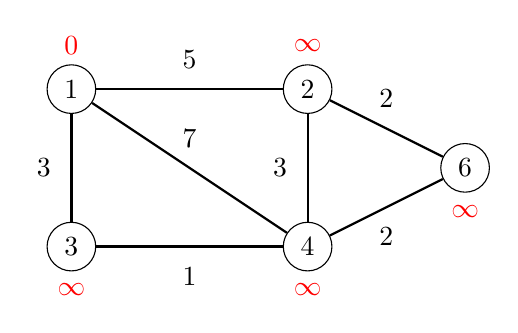
\begin{tikzpicture}
\node[draw, circle] (1) at (1,3) {1};
\node[draw, circle] (2) at (4,3) {2};
\node[draw, circle] (3) at (1,1) {3};
\node[draw, circle] (4) at (4,1) {4};
\node[draw, circle] (5) at (6,2) {6};
\node[color=red] at (1,3+0.55) {$0$};
\node[color=red] at (4,3+0.55) {$\infty$};
\node[color=red] at (1,1-0.55) {$\infty$};
\node[color=red] at (4,1-0.55) {$\infty$};
\node[color=red] at (6,2-0.55) {$\infty$};
\path[draw,thick,-] (1) -- node[font=\small,label=above:5] {} (2);
\path[draw,thick,-] (1) -- node[font=\small,label=left:3] {} (3);
\path[draw,thick,-] (3) -- node[font=\small,label=below:1] {} (4);
\path[draw,thick,-] (2) -- node[font=\small,label=left:3] {} (4);
\path[draw,thick,-] (2) -- node[font=\small,label=above:2] {} (5);
\path[draw,thick,-] (4) -- node[font=\small,label=below:2] {} (5);
\path[draw,thick,-] (1) -- node[font=\small,label=above:7] {} (4);
\end{tikzpicture}
\end{center}
به هر گره گراف یک فاصله نسبت داده می‌شود.
در ابتدا، فاصله تا گره مبدا برابر ۰ و فاصله تا سایر گره‌ها بی‌نهایت است.

الگوریتم یال‌هایی را جستجو می‌کند که فاصله‌ها را کاهش دهند.
ابتدا، تمام یال‌های خروجی از گره ۱ فاصله‌ها را کاهش می‌دهند:
\begin{center}
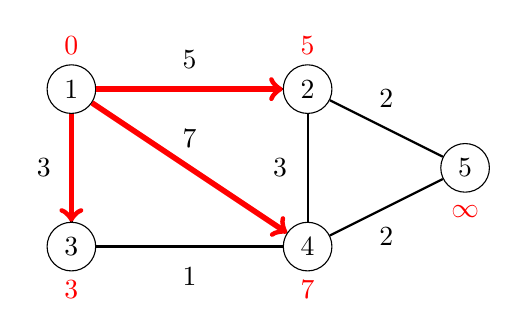
\begin{tikzpicture}
\node[draw, circle] (1) at (1,3) {1};
\node[draw, circle] (2) at (4,3) {2};
\node[draw, circle] (3) at (1,1) {3};
\node[draw, circle] (4) at (4,1) {4};
\node[draw, circle] (5) at (6,2) {5};
\node[color=red] at (1,3+0.55) {$0$};
\node[color=red] at (4,3+0.55) {$5$};
\node[color=red] at (1,1-0.55) {$3$};
\node[color=red] at (4,1-0.55) {$7$};
\node[color=red] at (6,2-0.55) {$\infty$};
\path[draw,thick,-] (1) -- node[font=\small,label=above:5] {} (2);
\path[draw,thick,-] (1) -- node[font=\small,label=left:3] {} (3);
\path[draw,thick,-] (3) -- node[font=\small,label=below:1] {} (4);
\path[draw,thick,-] (2) -- node[font=\small,label=left:3] {} (4);
\path[draw,thick,-] (2) -- node[font=\small,label=above:2] {} (5);
\path[draw,thick,-] (4) -- node[font=\small,label=below:2] {} (5);
\path[draw,thick,-] (1) -- node[font=\small,label=above:7] {} (4);

\path[draw=red,thick,->,line width=2pt] (1) -- (2);
\path[draw=red,thick,->,line width=2pt] (1) -- (3);
\path[draw=red,thick,->,line width=2pt] (1) -- (4);
\end{tikzpicture}
\end{center}
پس از این، یال‌های
$2 \rightarrow 5$ و $3 \rightarrow 4$
فاصله‌ها را کاهش می‌دهند:
\begin{center}
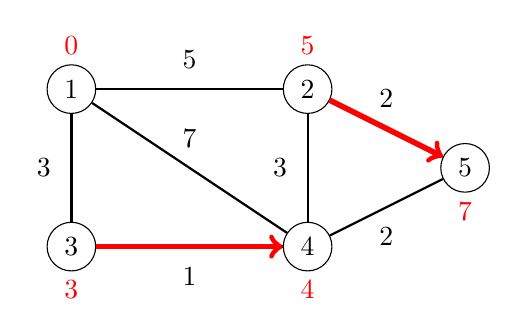
\begin{tikzpicture}
\node[draw, circle] (1) at (1,3) {1};
\node[draw, circle] (2) at (4,3) {2};
\node[draw, circle] (3) at (1,1) {3};
\node[draw, circle] (4) at (4,1) {4};
\node[draw, circle] (5) at (6,2) {5};
\node[color=red] at (1,3+0.55) {$0$};
\node[color=red] at (4,3+0.55) {$5$};
\node[color=red] at (1,1-0.55) {$3$};
\node[color=red] at (4,1-0.55) {$4$};
\node[color=red] at (6,2-0.55) {$7$};
\path[draw,thick,-] (1) -- node[font=\small,label=above:5] {} (2);
\path[draw,thick,-] (1) -- node[font=\small,label=left:3] {} (3);
\path[draw,thick,-] (3) -- node[font=\small,label=below:1] {} (4);
\path[draw,thick,-] (2) -- node[font=\small,label=left:3] {} (4);
\path[draw,thick,-] (2) -- node[font=\small,label=above:2] {} (5);
\path[draw,thick,-] (4) -- node[font=\small,label=below:2] {} (5);
\path[draw,thick,-] (1) -- node[font=\small,label=above:7] {} (4);

\path[draw=red,thick,->,line width=2pt] (2) -- (5);
\path[draw=red,thick,->,line width=2pt] (3) -- (4);
\end{tikzpicture}
\end{center}
در نهایت یک تغییر دیگر وجود دارد:
\begin{center}
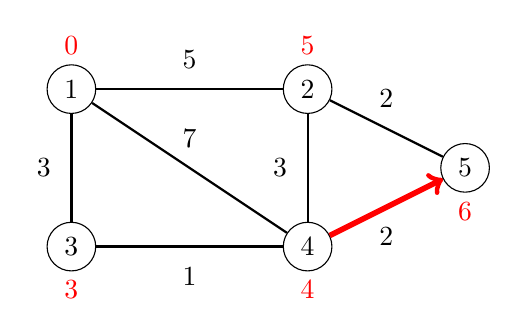
\begin{tikzpicture}
\node[draw, circle] (1) at (1,3) {1};
\node[draw, circle] (2) at (4,3) {2};
\node[draw, circle] (3) at (1,1) {3};
\node[draw, circle] (4) at (4,1) {4};
\node[draw, circle] (5) at (6,2) {5};
\node[color=red] at (1,3+0.55) {$0$};
\node[color=red] at (4,3+0.55) {$5$};
\node[color=red] at (1,1-0.55) {$3$};
\node[color=red] at (4,1-0.55) {$4$};
\node[color=red] at (6,2-0.55) {$6$};
\path[draw,thick,-] (1) -- node[font=\small,label=above:5] {} (2);
\path[draw,thick,-] (1) -- node[font=\small,label=left:3] {} (3);
\path[draw,thick,-] (3) -- node[font=\small,label=below:1] {} (4);
\path[draw,thick,-] (2) -- node[font=\small,label=left:3] {} (4);
\path[draw,thick,-] (2) -- node[font=\small,label=above:2] {} (5);
\path[draw,thick,-] (4) -- node[font=\small,label=below:2] {} (5);
\path[draw,thick,-] (1) -- node[font=\small,label=above:7] {} (4);

\path[draw=red,thick,->,line width=2pt] (4) -- (5);
\end{tikzpicture}
\end{center}

پس از این، هیچ یالی نمی‌تواند هیچ فاصله‌ای را کاهش دهد.
این یعنی فاصله‌ها نهایی هستند
و ما با موفقیت کوتاه‌ترین فاصله‌ها را
از گره آغازین به تمام گره‌های گراف محاسبه کرده‌ایم.

برای نمونه، کوتاه‌ترین فاصله 3
از گره 1 به گره 5 متناظر با
مسیر زیر است:

\begin{center}
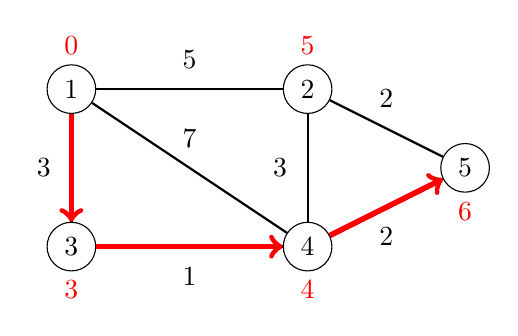
\begin{tikzpicture}
\node[draw, circle] (1) at (1,3) {1};
\node[draw, circle] (2) at (4,3) {2};
\node[draw, circle] (3) at (1,1) {3};
\node[draw, circle] (4) at (4,1) {4};
\node[draw, circle] (5) at (6,2) {5};
\node[color=red] at (1,3+0.55) {$0$};
\node[color=red] at (4,3+0.55) {$5$};
\node[color=red] at (1,1-0.55) {$3$};
\node[color=red] at (4,1-0.55) {$4$};
\node[color=red] at (6,2-0.55) {$6$};
\path[draw,thick,-] (1) -- node[font=\small,label=above:5] {} (2);
\path[draw,thick,-] (1) -- node[font=\small,label=left:3] {} (3);
\path[draw,thick,-] (3) -- node[font=\small,label=below:1] {} (4);
\path[draw,thick,-] (2) -- node[font=\small,label=left:3] {} (4);
\path[draw,thick,-] (2) -- node[font=\small,label=above:2] {} (5);
\path[draw,thick,-] (4) -- node[font=\small,label=below:2] {} (5);
\path[draw,thick,-] (1) -- node[font=\small,label=above:7] {} (4);

\path[draw=red,thick,->,line width=2pt] (1) -- (3);
\path[draw=red,thick,->,line width=2pt] (3) -- (4);
\path[draw=red,thick,->,line width=2pt] (4) -- (5);
\end{tikzpicture}
\end{center}

\subsubsection{پیاده‌سازی}

پیاده‌سازی زیر از الگوریتم بلمن–فورد
کوتاه‌ترین فاصله‌ها را از یک گره $x$ به تمام گره‌های گراف تعیین می‌کند.
کد فرض می‌کند گراف به‌صورت فهرست یال‌ها \texttt{edges}
شامل چندتایی‌هایی به شکل $(a,b,w)$ ذخیره شده است،
به این معنی که یالی از گره $a$ به گره $b$ با وزن $w$ وجود دارد.

این الگوریتم از $n-1$ دور تشکیل شده است
و در هر دور، تمام یال‌های گراف را بررسی کرده
و تلاش می‌کند فاصله‌ها را کاهش دهد.
الگوریتم یک آرایه \texttt{distance} می‌سازد
که شامل فاصله‌ها از $x$ به تمام رأس‌های گراف خواهد بود.
ثابت \texttt{INF} نشان‌دهنده فاصله بی‌نهایت است.

\begin{lstlisting}
for (int i = 1; i <= n; i++) distance[i] = INF;
distance[x] = 0;
for (int i = 1; i <= n-1; i++) {
    for (auto e : edges) {
        int a, b, w;
        tie(a, b, w) = e;
        distance[b] = min(distance[b], distance[a]+w);
    }
}
\end{lstlisting}

پیچیدگی زمانی الگوریتم $O(nm)$ است،
زیرا الگوریتم شامل $n-1$ دور است و
در طول یک دور روی تمام $m$ یال پیمایش می‌کند.
اگر هیچ دور منفی در گراف وجود نداشته باشد،
تمام فاصله‌ها پس از $n-1$ دور نهایی می‌شوند،
زیرا هر کوتاه‌ترین مسیر می‌تواند حداکثر شامل $n-1$ یال باشد.

در عمل، فاصله‌های نهایی معمولاً
سریع‌تر از $n-1$ دور پیدا می‌شوند.
بنابراین، یک روش ممکن برای افزایش کارایی الگوریتم
این است که اگر در طول یک دور هیچ فاصله‌ای کاهش نیافت،
اجرای الگوریتم متوقف شود.

\subsubsection{دورهای منفی}

\index{دور منفی}

الگوریتم بلمن-فورد همچنین می‌تواند برای
بررسی وجود دور با طول منفی در گراف به کار رود.
برای نمونه، گراف

\begin{center}
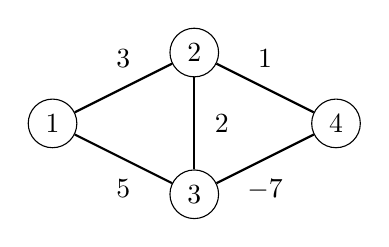
\begin{tikzpicture}[scale=0.9]
\node[draw, circle] (1) at (0,0) {$1$};
\node[draw, circle] (2) at (2,1) {$2$};
\node[draw, circle] (3) at (2,-1) {$3$};
\node[draw, circle] (4) at (4,0) {$4$};

\path[draw,thick,-] (1) -- node[font=\small,label=above:$3$] {} (2);
\path[draw,thick,-] (2) -- node[font=\small,label=above:$1$] {} (4);
\path[draw,thick,-] (1) -- node[font=\small,label=below:$5$] {} (3);
\path[draw,thick,-] (3) -- node[font=\small,label=below:$-7$] {} (4);
\path[draw,thick,-] (2) -- node[font=\small,label=right:$2$] {} (3);
\end{tikzpicture}
\end{center}
\noindent
شامل یک دور منفی
$2 \rightarrow 3 \rightarrow 4 \rightarrow 2$
با طول $-4$ است.

اگر گراف شامل دور منفی باشد،
می‌توان هر مسیری را که شامل این دور است،
با تکرار چندباره دور به تعداد نامتناهی کوتاه‌تر کرد.
بنابراین، مفهوم کوتاه‌ترین مسیر در این وضعیت معنایی ندارد.

یک دور منفی را می‌توان با اجرای الگوریتم بلمن-فورد
به مدت $n$ دور شناسایی کرد.
اگر دور آخر فاصله‌ای را کاهش دهد،
گراف شامل دور منفی است.
توجه کنید که این الگوریتم می‌تواند برای
یافتن دور منفی در کل گراف بدون توجه به رأس شروع استفاده شود.

\subsubsection{الگوریتم SPFA}

\index{الگوریتم SPFA}

\key{الگوریتم SPFA} (کوتاه‌ترین مسیر سریع‌تر) \cite{fan94}
گونه‌ای از الگوریتم بلمن-فورد است
که اغلب کارایی بیشتری نسبت به الگوریتم اصلی دارد.
الگوریتم SPFA در هر دور از تمام یال‌ها عبور نمی‌کند،
بلکه یال‌ها را برای بررسی به روش هوشمندانه‌تری انتخاب می‌کند.

این الگوریتم صف گره‌هایی که ممکن است برای کاهش فاصله‌ها استفاده شوند نگه می‌دارد.
ابتدا الگوریتم گره شروع $x$ را به صف اضافه می‌کند.
سپس همیشه اولین گره صف را پردازش می‌کند، و وقتی یال $a \rightarrow b$ فاصله‌ای را کاهش می‌دهد،
گره $b$ به صف اضافه می‌شود.
% 
% The following implementation uses a 
% \texttt{queue} \texttt{q}.
% In addition, an array \texttt{inqueue} indicates
% if a node is already in the queue,
% in which case the algorithm does not add
% the node to the queue again.
% 
% \begin{lstlisting}
% for (int i = 1; i <= n; i++) distance[i] = INF;
% distance[x] = 0;
% q.push(x);
% while (!q.empty()) {
%     int a = q.front(); q.pop();
%     inqueue[a] = false;
%     for (auto b : v[a]) {
%         if (distance[a]+b.second < distance[b.first]) {
%             distance[b.first] = distance[a]+b.second;
%             if (!inqueue[b]) {q.push(b); inqueue[b] = true;}
%         }
%     }
% }
% \end{lstlisting}

کارایی الگوریتم SPFA وابسته به ساختار گراف است:
الگوریتم اغلب کارا است،
اما بدترین پیچیدگی زمانی آن همچنان $O(nm)$ است و ساخت ورودی‌هایی که الگوریتم را به کندی الگوریتم اصلی بلمن-فورد کنند ممکن است.

\section{الگوریتم دایکسترا}

\index{الگوریتم دایکسترا}

\key{الگوریتم دایکسترا}\footnote{E. W. Dijkstra published the algorithm in 1959 \cite{dij59};
however, his original paper does not mention how to implement the algorithm efficiently.}
کوتاه‌ترین مسیرها از گره شروع به تمام گره‌های گراف را مثل الگوریتم بلمن-فورد پیدا می‌کند.
مزیت الگوریتم دایکسترا کارایی بالاتر و قابلیت پردازش گراف‌های بزرگ است.
با این حال، الگوریتم نبود یال با وزن منفی در گراف را شرط می‌داند.

مانند الگوریتم بلمن-فورد، الگوریتم دایکسترا فاصله‌ها تا گره‌ها را نگه می‌دارد و حین جستجو کاهش می‌دهد.
الگوریتم دایکسترا کارا است، چون با تکیه بر نبود یال‌های منفی، هر یال گراف را فقط یک بار پردازش می‌کند.

\subsubsection{مثال}

عملکرد الگوریتم دایکسترا در گراف زیر با شروع از گره ۱ را بررسی می‌کنیم:
\begin{center}
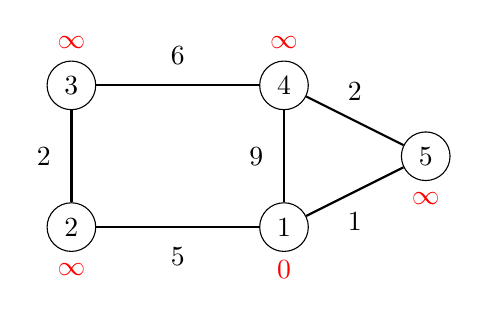
\begin{tikzpicture}[scale=0.9]
\node[draw, circle] (1) at (1,3) {3};
\node[draw, circle] (2) at (4,3) {4};
\node[draw, circle] (3) at (1,1) {2};
\node[draw, circle] (4) at (4,1) {1};
\node[draw, circle] (5) at (6,2) {5};

\node[color=red] at (1,3+0.6) {$\infty$};
\node[color=red] at (4,3+0.6) {$\infty$};
\node[color=red] at (1,1-0.6) {$\infty$};
\node[color=red] at (4,1-0.6) {$0$};
\node[color=red] at (6,2-0.6) {$\infty$};

\path[draw,thick,-] (1) -- node[font=\small,label=above:6] {} (2);
\path[draw,thick,-] (1) -- node[font=\small,label=left:2] {} (3);
\path[draw,thick,-] (3) -- node[font=\small,label=below:5] {} (4);
\path[draw,thick,-] (2) -- node[font=\small,label=left:9] {} (4);
\path[draw,thick,-] (2) -- node[font=\small,label=above:2] {} (5);
\path[draw,thick,-] (4) -- node[font=\small,label=below:1] {} (5);
\end{tikzpicture}
\end{center}
مشابه الگوریتم بلمن-فورد،
در ابتدا فاصله تا رأس آغازین ۰
و فاصله تا تمام رأس‌های دیگر بی‌نهایت است.

در هر گام، الگوریتم دایکسترا رأسی را انتخاب می‌کند
که هنوز پردازش نشده و فاصله‌اش
تا حد امکان کمینه است.
نخستین رأس با این مشخصه، رأس ۱ با فاصله ۰ است.

وقتی رأسی انتخاب شد، الگوریتم
تمام یال‌های خروجی از آن را بررسی می‌کند
و فاصله‌ها را به کمک آن‌ها کاهش می‌دهد:
\begin{center}
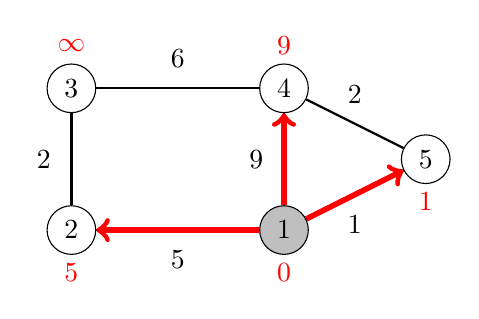
\begin{tikzpicture}[scale=0.9]
\node[draw, circle] (1) at (1,3) {3};
\node[draw, circle] (2) at (4,3) {4};
\node[draw, circle] (3) at (1,1) {2};
\node[draw, circle, fill=lightgray] (4) at (4,1) {1};
\node[draw, circle] (5) at (6,2) {5};

\node[color=red] at (1,3+0.6) {$\infty$};
\node[color=red] at (4,3+0.6) {$9$};
\node[color=red] at (1,1-0.6) {$5$};
\node[color=red] at (4,1-0.6) {$0$};
\node[color=red] at (6,2-0.6) {$1$};

\path[draw,thick,-] (1) -- node[font=\small,label=above:6] {} (2);
\path[draw,thick,-] (1) -- node[font=\small,label=left:2] {} (3);
\path[draw,thick,-] (3) -- node[font=\small,label=below:5] {} (4);
\path[draw,thick,-] (2) -- node[font=\small,label=left:9] {} (4);
\path[draw,thick,-] (2) -- node[font=\small,label=above:2] {} (5);
\path[draw,thick,-] (4) -- node[font=\small,label=below:1] {} (5);

\path[draw=red,thick,->,line width=2pt] (4) -- (2);
\path[draw=red,thick,->,line width=2pt] (4) -- (3);
\path[draw=red,thick,->,line width=2pt] (4) -- (5);
\end{tikzpicture}
\end{center}
در این حالت،
یال‌های رأس ۱ فاصله رأس‌های
۲، ۴ و ۵ را کاهش دادند؛ این فاصله‌ها اکنون ۵، ۹ و ۱ هستند.

رأس بعدی برای پردازش، رأس ۵ با فاصله ۱ است.
این انتخاب فاصله تا رأس ۴ را از ۹ به ۳ کاهش می‌دهد:
\begin{center}
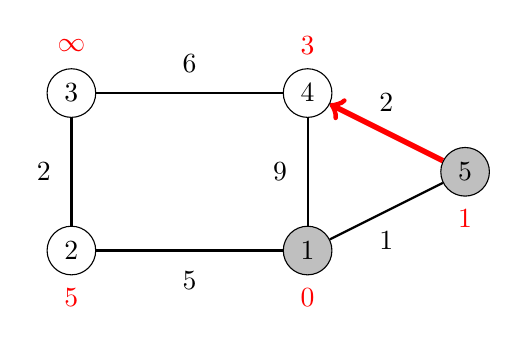
\begin{tikzpicture}
\node[draw, circle] (1) at (1,3) {3};
\node[draw, circle] (2) at (4,3) {4};
\node[draw, circle] (3) at (1,1) {2};
\node[draw, circle, fill=lightgray] (4) at (4,1) {1};
\node[draw, circle, fill=lightgray] (5) at (6,2) {5};

\node[color=red] at (1,3+0.6) {$\infty$};
\node[color=red] at (4,3+0.6) {$3$};
\node[color=red] at (1,1-0.6) {$5$};
\node[color=red] at (4,1-0.6) {$0$};
\node[color=red] at (6,2-0.6) {$1$};

\path[draw,thick,-] (1) -- node[font=\small,label=above:6] {} (2);
\path[draw,thick,-] (1) -- node[font=\small,label=left:2] {} (3);
\path[draw,thick,-] (3) -- node[font=\small,label=below:5] {} (4);
\path[draw,thick,-] (2) -- node[font=\small,label=left:9] {} (4);
\path[draw,thick,-] (2) -- node[font=\small,label=above:2] {} (5);
\path[draw,thick,-] (4) -- node[font=\small,label=below:1] {} (5);

\path[draw=red,thick,->,line width=2pt] (5) -- (2);
\end{tikzpicture}
\end{center}
پس از این، گره بعدی گره ۴ است که
فاصله تا گره ۳ را به ۹ کاهش می‌دهد:
\begin{center}
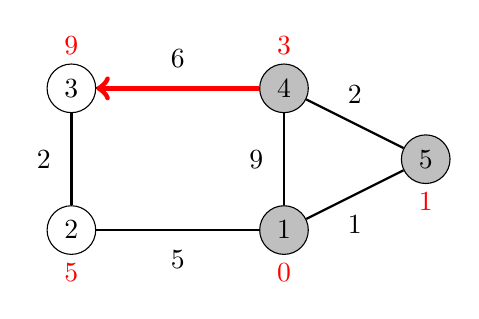
\begin{tikzpicture}[scale=0.9]
\node[draw, circle] (1) at (1,3) {3};
\node[draw, circle, fill=lightgray] (2) at (4,3) {4};
\node[draw, circle] (3) at (1,1) {2};
\node[draw, circle, fill=lightgray] (4) at (4,1) {1};
\node[draw, circle, fill=lightgray] (5) at (6,2) {5};

\node[color=red] at (1,3+0.6) {$9$};
\node[color=red] at (4,3+0.6) {$3$};
\node[color=red] at (1,1-0.6) {$5$};
\node[color=red] at (4,1-0.6) {$0$};
\node[color=red] at (6,2-0.6) {$1$};

\path[draw,thick,-] (1) -- node[font=\small,label=above:6] {} (2);
\path[draw,thick,-] (1) -- node[font=\small,label=left:2] {} (3);
\path[draw,thick,-] (3) -- node[font=\small,label=below:5] {} (4);
\path[draw,thick,-] (2) -- node[font=\small,label=left:9] {} (4);
\path[draw,thick,-] (2) -- node[font=\small,label=above:2] {} (5);
\path[draw,thick,-] (4) -- node[font=\small,label=below:1] {} (5);

\path[draw=red,thick,->,line width=2pt] (2) -- (1);
\end{tikzpicture}
\end{center}

ویژگی قابل توجه در الگوریتم دایکسترا این است که
هر زمان گره‌ای انتخاب شود، فاصله آن نهایی است.
برای نمونه، در این مرحله از الگوریتم،
فواصل ۰، ۱ و ۳ فواصل نهایی
تا گره‌های ۱، ۵ و ۴ هستند.

پس از این، الگوریتم دو گره باقی‌مانده
را پردازش می‌کند و فواصل نهایی به این صورت خواهند بود:

\begin{center}
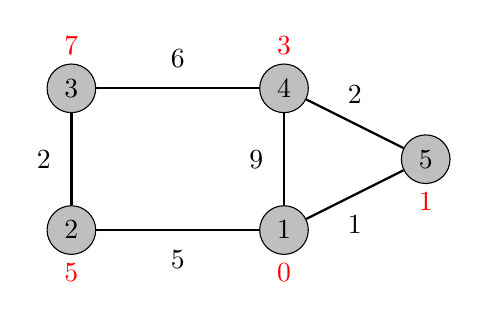
\begin{tikzpicture}[scale=0.9]
\node[draw, circle, fill=lightgray] (1) at (1,3) {3};
\node[draw, circle, fill=lightgray] (2) at (4,3) {4};
\node[draw, circle, fill=lightgray] (3) at (1,1) {2};
\node[draw, circle, fill=lightgray] (4) at (4,1) {1};
\node[draw, circle, fill=lightgray] (5) at (6,2) {5};

\node[color=red] at (1,3+0.6) {$7$};
\node[color=red] at (4,3+0.6) {$3$};
\node[color=red] at (1,1-0.6) {$5$};
\node[color=red] at (4,1-0.6) {$0$};
\node[color=red] at (6,2-0.6) {$1$};

\path[draw,thick,-] (1) -- node[font=\small,label=above:6] {} (2);
\path[draw,thick,-] (1) -- node[font=\small,label=left:2] {} (3);
\path[draw,thick,-] (3) -- node[font=\small,label=below:5] {} (4);
\path[draw,thick,-] (2) -- node[font=\small,label=left:9] {} (4);
\path[draw,thick,-] (2) -- node[font=\small,label=above:2] {} (5);
\path[draw,thick,-] (4) -- node[font=\small,label=below:1] {} (5);
\end{tikzpicture}
\end{center}

\subsubsection{یال‌های منفی}

کارایی الگوریتم دایکسترا مبتنی بر این است
که گراف یال منفی نداشته باشد.
اگر یال منفی وجود داشته باشد،
الگوریتم ممکن است نتایج نادرست بدهد.
به عنوان مثال، گراف زیر را در نظر بگیرید:

\begin{center}
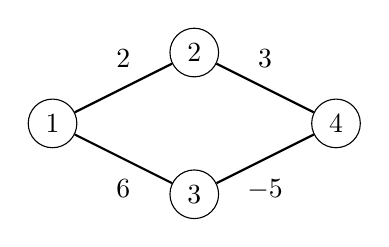
\begin{tikzpicture}[scale=0.9]
\node[draw, circle] (1) at (0,0) {$1$};
\node[draw, circle] (2) at (2,1) {$2$};
\node[draw, circle] (3) at (2,-1) {$3$};
\node[draw, circle] (4) at (4,0) {$4$};

\path[draw,thick,-] (1) -- node[font=\small,label=above:2] {} (2);
\path[draw,thick,-] (2) -- node[font=\small,label=above:3] {} (4);
\path[draw,thick,-] (1) -- node[font=\small,label=below:6] {} (3);
\path[draw,thick,-] (3) -- node[font=\small,label=below:$-5$] {} (4);
\end{tikzpicture}
\end{center}
\noindent
کوتاه‌ترین مسیر از رأس ۱ به رأس ۴ مسیر
$1 \rightarrow 3 \rightarrow 4$
با طول ۱ است.
با این حال، الگوریتم دایکسترا با دنبال کردن یال‌های با کمترین وزن،
مسیر $1 \rightarrow 2 \rightarrow 4$ را پیدا می‌کند.
این الگوریتم در نظر نمی‌گیرد که در مسیر دیگر،
وزن $-5$ وزن بزرگ قبلی یعنی ۶ را جبران می‌کند.

\subsubsection{پیاده‌سازی}

پیاده‌سازی زیر از الگوریتم دایکسترا،
کمترین فاصله از رأس $x$ به سایر رئوس گراف را محاسبه می‌کند.
گراف به صورت لیست‌های مجاورت ذخیره می‌شود به طوری که هرگاه یالی از رأس $a$ به رأس $b$ با وزن $w$ وجود داشته باشد،
\texttt{adj[$a$]} شامل جفت $(b,w)$ است.

پیاده‌سازی کارآمد الگوریتم دایکسترا نیازمند آن است که بتوان
رأس با کمترین فاصله را که هنوز پردازش نشده است، به صورت بهینه پیدا کرد.
داده‌ساختار مناسب برای این کار یک صف اولویت‌دار است
که رئوس را بر اساس فاصله‌شان مرتب نگه می‌دارد.
با استفاده از صف اولویت‌دار، رأس بعدی برای پردازش در زمان لگاریتمی قابل بازیابی است.

در کد زیر، صف اولویت‌دار \texttt{q} شامل جفت‌هایی به فرم $(-d,x)$ است؛
به این معنی که فاصله فعلی تا رأس $x$ برابر $d$ است.
آرایه $\texttt{distance}$ شامل فاصله تا هر رأس است و آرایه $\texttt{processed}$ نشان می‌دهد که آیا یک رأس پردازش شده است یا خیر.
در ابتدا فاصله تا $x$ برابر $0$ و برای سایر رئوس $\infty$ است.

\begin{lstlisting}
for (int i = 1; i <= n; i++) distance[i] = INF;
distance[x] = 0;
q.push({0,x});
while (!q.empty()) {
    int a = q.top().second; q.pop();
    if (processed[a]) continue;
    processed[a] = true;
    for (auto u : adj[a]) {
        int b = u.first, w = u.second;
        if (distance[a]+w < distance[b]) {
            distance[b] = distance[a]+w;
            q.push({-distance[b],b});
        }
    }
}
\end{lstlisting}

توجه کنید که صف اولویت‌دار شامل فاصله‌های \emph{منفی} تا رئوس است.
دلیل این موضوع این است که نسخه پیش‌فرض صف اولویت‌دار در C++،
بیشترین عنصر را پیدا می‌کند، در حالی که ما به دنبال کمترین عنصر هستیم.
با استفاده از فاصله‌های منفی، می‌توان مستقیماً از صف اولویت‌دار پیش‌فرض استفاده کرد\footnote{البته
می‌توانستیم صف اولویت‌دار را مشابه بخش ۴.۵ تعریف کرده و از فاصله‌های مثبت استفاده کنیم، اما پیاده‌سازی کمی طولانی‌تر می‌شد.}.
همچنین توجه داشته باشید که ممکن است چندین نمونه از یک رأس درون صف اولویت‌دار قرار گیرد؛
با این حال، فقط نمونه با کمترین فاصله پردازش خواهد شد.

پیچیدگی زمانی پیاده‌سازی فوق $O(n+m \log m)$ است،
زیرا الگوریتم تمام رئوس گراف را پیمایش کرده و به ازای هر یال،
حداکثر یک فاصله به صف اولویت‌دار اضافه می‌کند.

\section{الگوریتم فلوید-وارشال}

\index{الگوریتم فلوید-وارشال}

\key{الگوریتم فلوید–وارشال}\footnote{این الگوریتم به نام‌های آر. دبلیو. فلوید و اس. وارشال نام‌گذاری شده است که آن را به طور مستقل در سال ۱۹۶۲ منتشر کردند \cite{flo62,war62}.} رویکرد دیگری برای حل مسئله یافتن کوتاه‌ترین مسیرها ارائه می‌دهد. بر خلاف سایر الگوریتم‌های این فصل، این الگوریتم تمام کوتاه‌ترین مسیرهای بین گره‌ها را در یک بار اجرا پیدا می‌کند.

این الگوریتم یک آرایه دو‌بعدی شامل فاصله‌های بین گره‌ها را نگهداری می‌کند. ابتدا، فاصله‌ها فقط با استفاده از یال‌های مستقیم بین گره‌ها محاسبه می‌شوند، و پس از آن، الگوریتم با استفاده از گره‌های میانی در مسیرها، فاصله‌ها را کاهش می‌دهد.

\subsubsection{مثال}

نحوه کارکرد الگوریتم فلوید–وارشال را در گراف زیر بررسی می‌کنیم:

\begin{center}
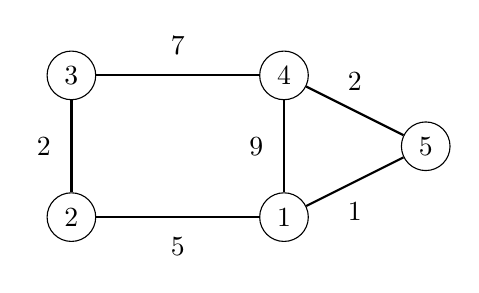
\begin{tikzpicture}[scale=0.9]
\node[draw, circle] (1) at (1,3) {$3$};
\node[draw, circle] (2) at (4,3) {$4$};
\node[draw, circle] (3) at (1,1) {$2$};
\node[draw, circle] (4) at (4,1) {$1$};
\node[draw, circle] (5) at (6,2) {$5$};

\path[draw,thick,-] (1) -- node[font=\small,label=above:7] {} (2);
\path[draw,thick,-] (1) -- node[font=\small,label=left:2] {} (3);
\path[draw,thick,-] (3) -- node[font=\small,label=below:5] {} (4);
\path[draw,thick,-] (2) -- node[font=\small,label=left:9] {} (4);
\path[draw,thick,-] (2) -- node[font=\small,label=above:2] {} (5);
\path[draw,thick,-] (4) -- node[font=\small,label=below:1] {} (5);
\end{tikzpicture}
\end{center}

در ابتدا، فاصله هر گره تا خودش برابر $0$ است، و اگر یالی با وزن $x$ بین گره‌های $a$ و $b$ وجود داشته باشد، فاصله بین این دو گره $x$ خواهد بود. سایر فاصله‌ها بی‌نهایت هستند.

در این گراف، آرایه اولیه به صورت زیر است:
\begin{center}
\begin{tabular}{r|rrrrr}
 & 1 & 2 & 3 & 4 & 5 \\
\hline
1 & 0 & 5 & $\infty$ & 9 & 1 \\
2 & 5 & 0 & 2 & $\infty$ & $\infty$ \\
3 & $\infty$ & 2 & 0 & 7 & $\infty$ \\
4 & 9 & $\infty$ & 7 & 0 & 2 \\
5 & 1 & $\infty$ & $\infty$ & 2 & 0 \\
\end{tabular}
\end{center}
\vspace{10pt}
الگوریتم شامل دورهای متوالی است. در هر دور، الگوریتم گره جدیدی را انتخاب می‌کند که از این پس می‌تواند به عنوان گره میانی در مسیرها عمل کند، و فاصله‌ها با استفاده از این گره کاهش می‌یابند.

در دور اول، گره ۱ گره میانی جدید است. یک مسیر جدید بین گره‌های ۲ و ۴ با طول ۱۴ پدید می‌آید، زیرا گره ۱ آن‌ها را به هم وصل می‌کند. همچنین یک مسیر جدید بین گره‌های ۲ و ۵ با طول ۶ ایجاد می‌شود.

\begin{center}
\begin{tabular}{r|rrrrr}
 & 1 & 2 & 3 & 4 & 5 \\
\hline
1 & 0 & 5 & $\infty$ & 9 & 1 \\
2 & 5 & 0 & 2 & \textbf{14} & \textbf{6} \\
3 & $\infty$ & 2 & 0 & 7 & $\infty$ \\
4 & 9 & \textbf{14} & 7 & 0 & 2 \\
5 & 1 & \textbf{6} & $\infty$ & 2 & 0 \\
\end{tabular}
\end{center}
\vspace{10pt}

در دور دوم، گره ۲ گره میانی جدید است. این کار مسیرهای جدیدی بین گره‌های ۱ و ۳ و بین گره‌های ۳ و ۵ ایجاد می‌کند:

\begin{center}
\begin{tabular}{r|rrrrr}
 & 1 & 2 & 3 & 4 & 5 \\
\hline
1 & 0 & 5 & \textbf{7} & 9 & 1 \\
2 & 5 & 0 & 2 & 14 & 6 \\
3 & \textbf{7} & 2 & 0 & 7 & \textbf{8} \\
4 & 9 & 14 & 7 & 0 & 2 \\
5 & 1 & 6 & \textbf{8} & 2 & 0 \\
\end{tabular}
\end{center}
\vspace{10pt}

در دور سوم، گره ۳ گره میانی جدید است.
مسیر جدیدی بین گره‌های ۲ و ۴ ایجاد می‌شود:

\begin{center}
\begin{tabular}{r|rrrrr}
 & 1 & 2 & 3 & 4 & 5 \\
\hline
1 & 0 & 5 & 7 & 9 & 1 \\
2 & 5 & 0 & 2 & \textbf{9} & 6 \\
3 & 7 & 2 & 0 & 7 & 8 \\
4 & 9 & \textbf{9} & 7 & 0 & 2 \\
5 & 1 & 6 & 8 & 2 & 0 \\
\end{tabular}
\end{center}
\vspace{10pt}

الگوریتم به همین ترتیب ادامه می‌یابد
تا زمانی که تمام گره‌ها به عنوان گره میانی تعیین شوند.
پس از پایان الگوریتم، آرایه شامل
کوتاه‌ترین فاصله‌ها بین هر دو گره است:

\begin{center}
\begin{tabular}{r|rrrrr}
 & 1 & 2 & 3 & 4 & 5 \\
\hline
1 & 0 & 5 & 7 & 3 & 1 \\
2 & 5 & 0 & 2 & 8 & 6 \\
3 & 7 & 2 & 0 & 7 & 8 \\
4 & 3 & 8 & 7 & 0 & 2 \\
5 & 1 & 6 & 8 & 2 & 0 \\
\end{tabular}
\end{center}

برای مثال، آرایه نشان می‌دهد که
کوتاه‌ترین فاصله بین گره‌های ۲ و ۴ برابر ۸ است.
این متناظر با مسیر زیر است:

\begin{center}
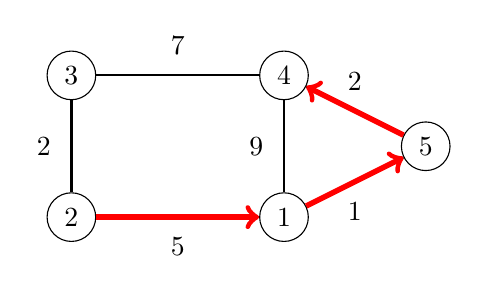
\begin{tikzpicture}[scale=0.9]
\node[draw, circle] (1) at (1,3) {$3$};
\node[draw, circle] (2) at (4,3) {$4$};
\node[draw, circle] (3) at (1,1) {$2$};
\node[draw, circle] (4) at (4,1) {$1$};
\node[draw, circle] (5) at (6,2) {$5$};

\path[draw,thick,-] (1) -- node[font=\small,label=above:7] {} (2);
\path[draw,thick,-] (1) -- node[font=\small,label=left:2] {} (3);
\path[draw,thick,-] (3) -- node[font=\small,label=below:5] {} (4);
\path[draw,thick,-] (2) -- node[font=\small,label=left:9] {} (4);
\path[draw,thick,-] (2) -- node[font=\small,label=above:2] {} (5);
\path[draw,thick,-] (4) -- node[font=\small,label=below:1] {} (5);

\path[draw=red,thick,->,line width=2pt] (3) -- (4);
\path[draw=red,thick,->,line width=2pt] (4) -- (5);
\path[draw=red,thick,->,line width=2pt] (5) -- (2);
\end{tikzpicture}
\end{center}

\subsubsection{پیاده‌سازی}

مزیت الگوریتم فلوید-وارشال
سادگی پیاده‌سازی آن است.
کد زیر ماتریس فاصله‌ای می‌سازد که در آن $\texttt{distance}[a][b]$
کوتاه‌ترین فاصله بین گره‌های $a$ و $b$ است.
ابتدا، الگوریتم \texttt{distance} را
با استفاده از ماتریس مجاورت \texttt{adj} گراف مقداردهی اولیه می‌کند:

\begin{lstlisting}
for (int i = 1; i <= n; i++) {
    for (int j = 1; j <= n; j++) {
        if (i == j) distance[i][j] = 0;
        else if (adj[i][j]) distance[i][j] = adj[i][j];
        else distance[i][j] = INF;
    }
}
\end{lstlisting}
سپس، کوتاه‌ترین فاصله‌ها به صورت زیر محاسبه می‌شوند:
\begin{lstlisting}
for (int k = 1; k <= n; k++) {
    for (int i = 1; i <= n; i++) {
        for (int j = 1; j <= n; j++) {
            distance[i][j] = min(distance[i][j],
                                   distance[i][k]+distance[k][j]);
        }
    }
}
\end{lstlisting}

پیچیدگی زمانی الگوریتم $O(n^3)$ است، زیرا شامل سه حلقه تو‌در‌تو است که روی رأس‌های گراف پیمایش می‌کنند.

از آنجا که پیاده‌سازی الگوریتم فلوید-وارشال ساده است، حتی اگر فقط پیدا کردن یک کوتاه‌ترین مسیر در گراف نیاز باشد، این الگوریتم می‌تواند انتخاب خوبی باشد. با این حال، الگوریتم تنها زمانی قابل استفاده است که گراف به اندازه‌ای کوچک باشد که پیچیدگی زمانی مکعبی برای آن به اندازه کافی سریع باشد.